
%% bare_conf.tex
%% V1.3
%% 2007/01/11
%% by Michael Shell
%% See:
%% http://www.michaelshell.org/
%% for current contact information.
%%
%% This is a skeleton file demonstrating the use of IEEEtran.cls
%% (requires IEEEtran.cls version 1.7 or later) with an IEEE conference paper.
%%
%% Support sites:
%% http://www.michaelshell.org/tex/ieeetran/
%% http://www.ctan.org/tex-archive/macros/latex/contrib/IEEEtran/
%% and
%% http://www.ieee.org/

%%*************************************************************************
%% Legal Notice:
%% This code is offered as-is without any warranty either expressed or
%% implied; without even the implied warranty of MERCHANTABILITY or
%% FITNESS FOR A PARTICULAR PURPOSE! 
%% User assumes all risk.
%% In no event shall IEEE or any contributor to this code be liable for
%% any damages or losses, including, but not limited to, incidental,
%% consequential, or any other damages, resulting from the use or misuse
%% of any information contained here.
%%
%% All comments are the opinions of their respective authors and are not
%% necessarily endorsed by the IEEE.
%%
%% This work is distributed under the LaTeX Project Public License (LPPL)
%% ( http://www.latex-project.org/ ) version 1.3, and may be freely used,
%% distributed and modified. A copy of the LPPL, version 1.3, is included
%% in the base LaTeX documentation of all distributions of LaTeX released
%% 2003/12/01 or later.
%% Retain all contribution notices and credits.
%% ** Modified files should be clearly indicated as such, including  **
%% ** renaming them and changing author support contact information. **
%%
%% File list of work: IEEEtran.cls, IEEEtran_HOWTO.pdf, bare_adv.tex,
%%                    bare_conf.tex, bare_jrnl.tex, bare_jrnl_compsoc.tex
%%*************************************************************************

% *** Authors should verify (and, if needed, correct) their LaTeX system  ***
% *** with the testflow diagnostic prior to trusting their LaTeX platform ***
% *** with production work. IEEE's font choices can trigger bugs that do  ***
% *** not appear when using other class files.                            ***
% The testflow support page is at:
% http://www.michaelshell.org/tex/testflow/



% Note that the a4paper option is mainly intended so that authors in
% countries using A4 can easily print to A4 and see how their papers will
% look in print - the typesetting of the document will not typically be
% affected with changes in paper size (but the bottom and side margins will).
% Use the testflow package mentioned above to verify correct handling of
% both paper sizes by the user's LaTeX system.
%
% Also note that the "draftcls" or "draftclsnofoot", not "draft", option
% should be used if it is desired that the figures are to be displayed in
% draft mode.
%
\documentclass[conference]{IEEEtran}
% Add the compsoc option for Computer Society conferences.
%
% If IEEEtran.cls has not been installed into the LaTeX system files,
% manually specify the path to it like:
% \documentclass[conference]{../sty/IEEEtran}





% Some very useful LaTeX packages include:
% (uncomment the ones you want to load)


% *** MISC UTILITY PACKAGES ***
%
%\usepackage{ifpdf}
% Heiko Oberdiek's ifpdf.sty is very useful if you need conditional
% compilation based on whether the output is pdf or dvi.
% usage:
% \ifpdf
%   % pdf code
% \else
%   % dvi code
% \fi
% The latest version of ifpdf.sty can be obtained from:
% http://www.ctan.org/tex-archive/macros/latex/contrib/oberdiek/
% Also, note that IEEEtran.cls V1.7 and later provides a builtin
% \ifCLASSINFOpdf conditional that works the same way.
% When switching from latex to pdflatex and vice-versa, the compiler may
% have to be run twice to clear warning/error messages.






% *** CITATION PACKAGES ***
%
%\usepackage{cite}
% cite.sty was written by Donald Arseneau
% V1.6 and later of IEEEtran pre-defines the format of the cite.sty package
% \cite{} output to follow that of IEEE. Loading the cite package will
% result in citation numbers being automatically sorted and properly
% "compressed/ranged". e.g., [1], [9], [2], [7], [5], [6] without using
% cite.sty will become [1], [2], [5]--[7], [9] using cite.sty. cite.sty's
% \cite will automatically add leading space, if needed. Use cite.sty's
% noadjust option (cite.sty V3.8 and later) if you want to turn this off.
% cite.sty is already installed on most LaTeX systems. Be sure and use
% version 4.0 (2003-05-27) and later if using hyperref.sty. cite.sty does
% not currently provide for hyperlinked citations.
% The latest version can be obtained at:
% http://www.ctan.org/tex-archive/macros/latex/contrib/cite/
% The documentation is contained in the cite.sty file itself.






% *** GRAPHICS RELATED PACKAGES ***
%
\ifCLASSINFOpdf
\usepackage[pdftex]{graphicx}
\usepackage{amsmath}
\usepackage{float}
\usepackage{enumerate}
\usepackage{listings}
\usepackage{url}
\usepackage{multirow}
\usepackage{fmtcount}

  % declare the path(s) where your graphic files are
  % \graphicspath{{../pdf/}{../jpeg/}}
  % and their extensions so you won't have to specify these with
  % every instance of \includegraphics
  % \DeclareGraphicsExtensions{.pdf,.jpeg,.png}
\else
  % or other class option (dvipsone, dvipdf, if not using dvips). graphicx
  % will default to the driver specified in the system graphics.cfg if no
  % driver is specified.
  % \usepackage[dvips]{graphicx}
  % declare the path(s) where your graphic files are
  % \graphicspath{{../eps/}}
  % and their extensions so you won't have to specify these with
  % every instance of \includegraphics
  % \DeclareGraphicsExtensions{.eps}
\fi
% graphicx was written by David Carlisle and Sebastian Rahtz. It is
% required if you want graphics, photos, etc. graphicx.sty is already
% installed on most LaTeX systems. The latest version and documentation can
% be obtained at: 
% http://www.ctan.org/tex-archive/macros/latex/required/graphics/
% Another good source of documentation is "Using Imported Graphics in
% LaTeX2e" by Keith Reckdahl which can be found as epslatex.ps or
% epslatex.pdf at: http://www.ctan.org/tex-archive/info/
%
% latex, and pdflatex in dvi mode, support graphics in encapsulated
% postscript (.eps) format. pdflatex in pdf mode supports graphics
% in .pdf, .jpeg, .png and .mps (metapost) formats. Users should ensure
% that all non-photo figures use a vector format (.eps, .pdf, .mps) and
% not a bitmapped formats (.jpeg, .png). IEEE frowns on bitmapped formats
% which can result in "jaggedy"/blurry rendering of lines and letters as
% well as large increases in file sizes.
%
% You can find documentation about the pdfTeX application at:
% http://www.tug.org/applications/pdftex





% *** MATH PACKAGES ***
%
%\usepackage[cmex10]{amsmath}
% A popular package from the American Mathematical Society that provides
% many useful and powerful commands for dealing with mathematics. If using
% it, be sure to load this package with the cmex10 option to ensure that
% only type 1 fonts will utilized at all point sizes. Without this option,
% it is possible that some math symbols, particularly those within
% footnotes, will be rendered in bitmap form which will result in a
% document that can not be IEEE Xplore compliant!
%
% Also, note that the amsmath package sets \interdisplaylinepenalty to 10000
% thus preventing page breaks from occurring within multiline equations. Use:
%\interdisplaylinepenalty=2500
% after loading amsmath to restore such page breaks as IEEEtran.cls normally
% does. amsmath.sty is already installed on most LaTeX systems. The latest
% version and documentation can be obtained at:
% http://www.ctan.org/tex-archive/macros/latex/required/amslatex/math/





% *** SPECIALIZED LIST PACKAGES ***
%
%\usepackage{algorithmic}
% algorithmic.sty was written by Peter Williams and Rogerio Brito.
% This package provides an algorithmic environment fo describing algorithms.
% You can use the algorithmic environment in-text or within a figure
% environment to provide for a floating algorithm. Do NOT use the algorithm
% floating environment provided by algorithm.sty (by the same authors) or
% algorithm2e.sty (by Christophe Fiorio) as IEEE does not use dedicated
% algorithm float types and packages that provide these will not provide
% correct IEEE style captions. The latest version and documentation of
% algorithmic.sty can be obtained at:
% http://www.ctan.org/tex-archive/macros/latex/contrib/algorithms/
% There is also a support site at:
% http://algorithms.berlios.de/index.html
% Also of interest may be the (relatively newer and more customizable)
% algorithmicx.sty package by Szasz Janos:
% http://www.ctan.org/tex-archive/macros/latex/contrib/algorithmicx/




% *** ALIGNMENT PACKAGES ***
%
%\usepackage{array}
% Frank Mittelbach's and David Carlisle's array.sty patches and improves
% the standard LaTeX2e array and tabular environments to provide better
% appearance and additional user controls. As the default LaTeX2e table
% generation code is lacking to the point of almost being broken with
% respect to the quality of the end results, all users are strongly
% advised to use an enhanced (at the very least that provided by array.sty)
% set of table tools. array.sty is already installed on most systems. The
% latest version and documentation can be obtained at:
% http://www.ctan.org/tex-archive/macros/latex/required/tools/


%\usepackage{mdwmath}
%\usepackage{mdwtab}
% Also highly recommended is Mark Wooding's extremely powerful MDW tools,
% especially mdwmath.sty and mdwtab.sty which are used to format equations
% and tables, respectively. The MDWtools set is already installed on most
% LaTeX systems. The lastest version and documentation is available at:
% http://www.ctan.org/tex-archive/macros/latex/contrib/mdwtools/


% IEEEtran contains the IEEEeqnarray family of commands that can be used to
% generate multiline equations as well as matrices, tables, etc., of high
% quality.


%\usepackage{eqparbox}
% Also of notable interest is Scott Pakin's eqparbox package for creating
% (automatically sized) equal width boxes - aka "natural width parboxes".
% Available at:
% http://www.ctan.org/tex-archive/macros/latex/contrib/eqparbox/





% *** SUBFIGURE PACKAGES ***
%\usepackage[tight,footnotesize]{subfigure}
% subfigure.sty was written by Steven Douglas Cochran. This package makes it
% easy to put subfigures in your figures. e.g., "Figure 1a and 1b". For IEEE
% work, it is a good idea to load it with the tight package option to reduce
% the amount of white space around the subfigures. subfigure.sty is already
% installed on most LaTeX systems. The latest version and documentation can
% be obtained at:
% http://www.ctan.org/tex-archive/obsolete/macros/latex/contrib/subfigure/
% subfigure.sty has been superceeded by subfig.sty.



%\usepackage[caption=false]{caption}
%\usepackage[font=footnotesize]{subfig}
% subfig.sty, also written by Steven Douglas Cochran, is the modern
% replacement for subfigure.sty. However, subfig.sty requires and
% automatically loads Axel Sommerfeldt's caption.sty which will override
% IEEEtran.cls handling of captions and this will result in nonIEEE style
% figure/table captions. To prevent this problem, be sure and preload
% caption.sty with its "caption=false" package option. This is will preserve
% IEEEtran.cls handing of captions. Version 1.3 (2005/06/28) and later 
% (recommended due to many improvements over 1.2) of subfig.sty supports
% the caption=false option directly:
%\usepackage[caption=false,font=footnotesize]{subfig}
%
% The latest version and documentation can be obtained at:
% http://www.ctan.org/tex-archive/macros/latex/contrib/subfig/
% The latest version and documentation of caption.sty can be obtained at:
% http://www.ctan.org/tex-archive/macros/latex/contrib/caption/




% *** FLOAT PACKAGES ***
%
%\usepackage{fixltx2e}
% fixltx2e, the successor to the earlier fix2col.sty, was written by
% Frank Mittelbach and David Carlisle. This package corrects a few problems
% in the LaTeX2e kernel, the most notable of which is that in current
% LaTeX2e releases, the ordering of single and double column floats is not
% guaranteed to be preserved. Thus, an unpatched LaTeX2e can allow a
% single column figure to be placed prior to an earlier double column
% figure. The latest version and documentation can be found at:
% http://www.ctan.org/tex-archive/macros/latex/base/



%\usepackage{stfloats}
% stfloats.sty was written by Sigitas Tolusis. This package gives LaTeX2e
% the ability to do double column floats at the bottom of the page as well
% as the top. (e.g., "\begin{figure*}[!b]" is not normally possible in
% LaTeX2e). It also provides a command:
%\fnbelowfloat
% to enable the placement of footnotes below bottom floats (the standard
% LaTeX2e kernel puts them above bottom floats). This is an invasive package
% which rewrites many portions of the LaTeX2e float routines. It may not work
% with other packages that modify the LaTeX2e float routines. The latest
% version and documentation can be obtained at:
% http://www.ctan.org/tex-archive/macros/latex/contrib/sttools/
% Documentation is contained in the stfloats.sty comments as well as in the
% presfull.pdf file. Do not use the stfloats baselinefloat ability as IEEE
% does not allow \baselineskip to stretch. Authors submitting work to the
% IEEE should note that IEEE rarely uses double column equations and
% that authors should try to avoid such use. Do not be tempted to use the
% cuted.sty or midfloat.sty packages (also by Sigitas Tolusis) as IEEE does
% not format its papers in such ways.





% *** PDF, URL AND HYPERLINK PACKAGES ***
%
%\usepackage{url}
% url.sty was written by Donald Arseneau. It provides better support for
% handling and breaking URLs. url.sty is already installed on most LaTeX
% systems. The latest version can be obtained at:
% http://www.ctan.org/tex-archive/macros/latex/contrib/misc/
% Read the url.sty source comments for usage information. Basically,
% \url{my_url_here}.





% *** Do not adjust lengths that control margins, column widths, etc. ***
% *** Do not use packages that alter fonts (such as pslatex).         ***
% There should be no need to do such things with IEEEtran.cls V1.6 and later.
% (Unless specifically asked to do so by the journal or conference you plan
% to submit to, of course. )


% correct bad hyphenation here
\hyphenation{op-tical net-works semi-conduc-tor}


\begin{document}
%
% paper title
% can use linebreaks \\ within to get better formatting as desired
\title{Ontology Models of OpenStack IaaS Architectures}


% author names and affiliations
% use a multiple column layout for up to three different
% affiliations
\author{\IEEEauthorblockN{Ales Komarek}
\IEEEauthorblockA{Faculty of Informatics and Management\\
University of Hradec Kralove\\ Czech Republic\\
Email: ales.komarek@uhk.cz}
\and
\IEEEauthorblockN{Jakub Pavlik}
\IEEEauthorblockA{Faculty of Informatics and Management\\
University of Hradec Kralove\\ Czech Republic\\
Email: jakub.pavlik.7@uhk.cz}
\and
\IEEEauthorblockN{Vladimir Sobeslav}
\IEEEauthorblockA{Faculty of Informatics and Management\\
University of Hradec Kralove\\ Czech Republic\\
Email: vladimir.sobeslav@uhk.cz}}

% conference papers do not typically use \thanks and this command
% is locked out in conference mode. If really needed, such as for
% the acknowledgment of grants, issue a \IEEEoverridecommandlockouts
% after \documentclass

% for over three affiliations, or if they all won't fit within the width
% of the page, use this alternative format:
% 
%\author{\IEEEauthorblockN{Michael Shell\IEEEauthorrefmark{1},
%Homer Simpson\IEEEauthorrefmark{2},
%James Kirk\IEEEauthorrefmark{3}, 
%Montgomery Scott\IEEEauthorrefmark{3} and
%Eldon Tyrell\IEEEauthorrefmark{4}}
%\IEEEauthorblockA{\IEEEauthorrefmark{1}School of Electrical and Computer Engineering\\
%Georgia Institute of Technology,
%Atlanta, Georgia 30332--0250\\ Email: see http://www.michaelshell.org/contact.html}
%\IEEEauthorblockA{\IEEEauthorrefmark{2}Twentieth Century Fox, Springfield, USA\\
%Email: homer@thesimpsons.com}
%\IEEEauthorblockA{\IEEEauthorrefmark{3}Starfleet Academy, San Francisco, California 96678-2391\\
%Telephone: (800) 555--1212, Fax: (888) 555--1212}
%\IEEEauthorblockA{\IEEEauthorrefmark{4}Tyrell Inc., 123 Replicant Street, Los Angeles, California 90210--4321}}

% use for special paper notices
%\IEEEspecialpapernotice{(Invited Paper)}

% make the title area
\maketitle

\begin{abstract}

%\boldmath

This paper explains how ontology can be used to model various OpenStack architectures. OpenStack is the largest open source cloud computing IaaS platform. It has been gaining wide spread popularity among users as well as software and hardware vendors over past few years. It's a very flexible system that can support a wide range of virtualization scenarios at any scale.

In our work we propose a formalization of OpenStack architectural model that can be automatically validated and serve suitable meta-data to configuration management tools. The OWL-DL based ontology defines service components and their relations and  provides foundation for further reasoning. Provided models can support simple all-in-one architecture as as well as large architectures with service components in High Availability setup.

\end{abstract}

% no keywords

% For peer review papers, you can put extra information on the cover
% page as needed:
% \ifCLASSOPTIONpeerreview
% \begin{center} \bfseries EDICS Category: 3-BBND \end{center}
% \fi
%
% For peerreview papers, this IEEEtran command inserts a page break and
% creates the second title. It will be ignored for other modes.
\IEEEpeerreviewmaketitle


\section{Introduction}

%proč OpenStack - protože komunita 500000 vývojářů, tisíce firem, nárůst kódu za poslední dobu stacalytics.com 
% How OpenStack Works?

%vendor lockin, scalability from notebook to thousans of servers like CERN

% 2,292 Companies; 8,066 Individual Members; 130 Countries; 2,007 Total Contributors; 341 Average Monthly Contributors; 89,156 Code Contributors - more information at 
% www.stackalytics.com July 2014

OpenStack is the largest open-source cloud computing platform today. Many companies participate to its code, extend core functions and write new service backends to fit their business goals. The actual system consists of many components designed with plugin architecture that allows custom implementations for various service backends. These components can be combined and configured to match available software and hardware resources and real use-case needs.

Each implementation has its own component combination and use some form of configuration management tool to enforce the service states on designated servers and possibly other network components. These tools require data that covers configuration of all components. Detecting component inconsistencies by hand is painful and time consuming process.

We propose a formalization of OpenStack service architecture model, based on the approaches developed in classic knowledge representation domain, especially Service-Oriented Architecture by OpenGroup. Component definition is encoded in an ontology using the standard OWL-DL language, which enables sharing of knowledge about configurations across various systems. Reasoning can be used on the specification to automate validation of configuration changes.

When dealing with hundreds of components with thousands of properties and relations, keeping track of changes throughout its life cycle is very challenging. Current approaches are ad hoc, even OpenStack Fuel has severe limitations, there exists no standard for specifying common OpenStack architectural model. The question how to convert the proposed OWL-DL schema to metadata format that configuration management tools can process is discussed. We are working on external node classification service that uses graph database to serialize the OWL ontology with REST API that configuration management tools can use as metadata provider. This can streamline the process of adopting new services and service backends in predictable manner.

\subsection{Use Cases}

OpenStack is system that has growing number of components with growing number of components and drivers. As we will show in following text there's no universal installation of OpenStack.  

% představit OpenStack jako systém s rolemi, konfiguracemi, komponenty, drivery. jina instalace per use case. Nexexistuje univerzální instalace. Vysoka komplexita, services

\subsection{Infrastructure Modeling}

Tools usually collect required metadata through web forms or answer files. This is not a conceptual way to describe model.

% Jak vytvořit high level model (logické schéma) architektury? a přenést ji do low level design realizace? 
% Jak správně definovat architekturu na základě hw infrastruktury a target use case?

\subsection{Process Automation}

% Jak celý proces deploymentu automatizovat?



\section{Architectural Models}

Jak funguje IaaS ve smyslu deploye masiny z pohledu controlleru - zavola scheduler, ten comupte, ten pak glance, pak pripadne cinder a neutron a pusti boot, kdyz to ma ready. a tim padem provoz.

obzrazel

\subsection{Architectural Level}

OpenStack is complete Infrastructure as a Service platforms. It allows to create virtual servers on virtual networks using virtual block devices. These core services are followed by growing number of services covering for example telemetry, orchestration or data processing. All services within OpenStack architecture have pluggable backends. This allows vendors to develop plugin for their resources, that can be accessed and managed by the OpenStack API.

Figure X shows the basic configuration of OpenStack in Icehouse version.

Klasicky logicky model openstack architektury

2) OpenStack architecture moduls

Rozebrat services a představit modularitu a vendor plugins, drivers

Database

Message queue

Time service

Identity - Keystone

Image - Glance

Compute - Nova

Network - Neutron

Volume - Cinder

\subsection{Solution level}

Real implementations of Architectural models

\subsubsection{IaaS controller support}

Cluster software
- corosync/pacemaker
- keepalived

Database
- mysql/galera
- postgressql/xtradb

RPC
- rabbitmq
- qpid
- 0mq

time

\subsubsection{Iaas Controller services}

Pluggable backends

Keystone
- file
- sql
- ldap

Glance
- dir
- swift

Nova
- kvm
- qemu
- docker
- hyper-v

Neutron
- flat
- ovs-gre/vxlan
- sdns

Cinder
- lvms
- sans


Různé způsoby nasazení ukázky reálné architektury - promapovat ve 4 na ontologii

\subsection{Hardware matters}

Why we choose different openstack setups

Lab1 - 20 hypervisors, kvm, ovs-gre, local hdd
Lab2 - 4 hypervisoers, kvm, sdn-contrail, san
Lab3 - 5 hypervisors, ...



\section{OpenStack Deployment Options}

There are many ways how to deploy OpenStack infrastructure which are more or less automated. Some of them require to fill in answer files, some configuration files. Some tools have graphiceal user interface and allow to provision entire hardware infrastructure as some just configure the services on the provisioned servers.

Model je popsanej dokumentem a není to čitelný, automatizace. Není validita modelu. Chyby se debugují na úrovni reality.

\subsection{Development Environment Installers}

For testing and developing OpenStack ...

\subsubsection{PackStack}

Packstack is a utility that uses Puppet modules to deploy various parts of OpenStack on multiple pre-installed servers over SSH automatically. Currently only Fedora, Red Hat Enterprise Linux (RHEL) and compatible derivatives of both are supported.

% https://wiki.openstack.org/wiki/Packstack

\subsubsection{Devstack}

DevStack has evolved to support a large number of configuration options and alternative platforms and support services. That evolution has grown well beyond what was originally intended and the majority of configuration combinations are rarely, if ever, tested.

% http://devstack.org/overview.html

\subsection{Production Environment Managers}

For production installations of OpenStack ...

\subsubsection{Fuel}

Fuel is an open source deployment and management tool for OpenStack. Developed as an OpenStack community effort, it provides an intuitive, GUI-driven experience for deployment and management of OpenStack, related community projects and plug-ins. 

% https://wiki.openstack.org/wiki/Fuel

\subsubsection{Foreman}

You can setup Foreman to deploy RDO. The metadata is provided in Host Groups.

% https://openstack.redhat.com/Deploying_RDO_using_Foreman

\subsection{Configuration Management Tools}

You can install OpenStack by configuration management tool

\subsubsection{Puppet}

It's already used by Fuel an Foreman

\subsubsection{Salt}

Salt is another approach to install OpenStack.


\section{Ontology of OpenStack System}

\subsection{Serialization Formats}

Způsoby serialiazce ontologie

\subsubsection{XML Documents}

RDF format

\subsubsection{Graph databases}

Preserving RDF format, just very different implementation 

je to servica, tzn overhead oproti xml filu, ale zas ma api atd ...

\subsubsection{Hierarchical}

Subject (id) or property driven

\subsection{Comparison}

Srovnání jednolivých formátů pro ontologii pro openstack řešení - bezpečnost, rychlost, integrace

- speed - parsing / scaling
- integration, maintenance costs
- security issues



\section{Ontology Usage}

We chose the Opengroup's Service Oriented Architecture as a 

\subsection{Ontology details}

\begin{figure}[!h]
\centering
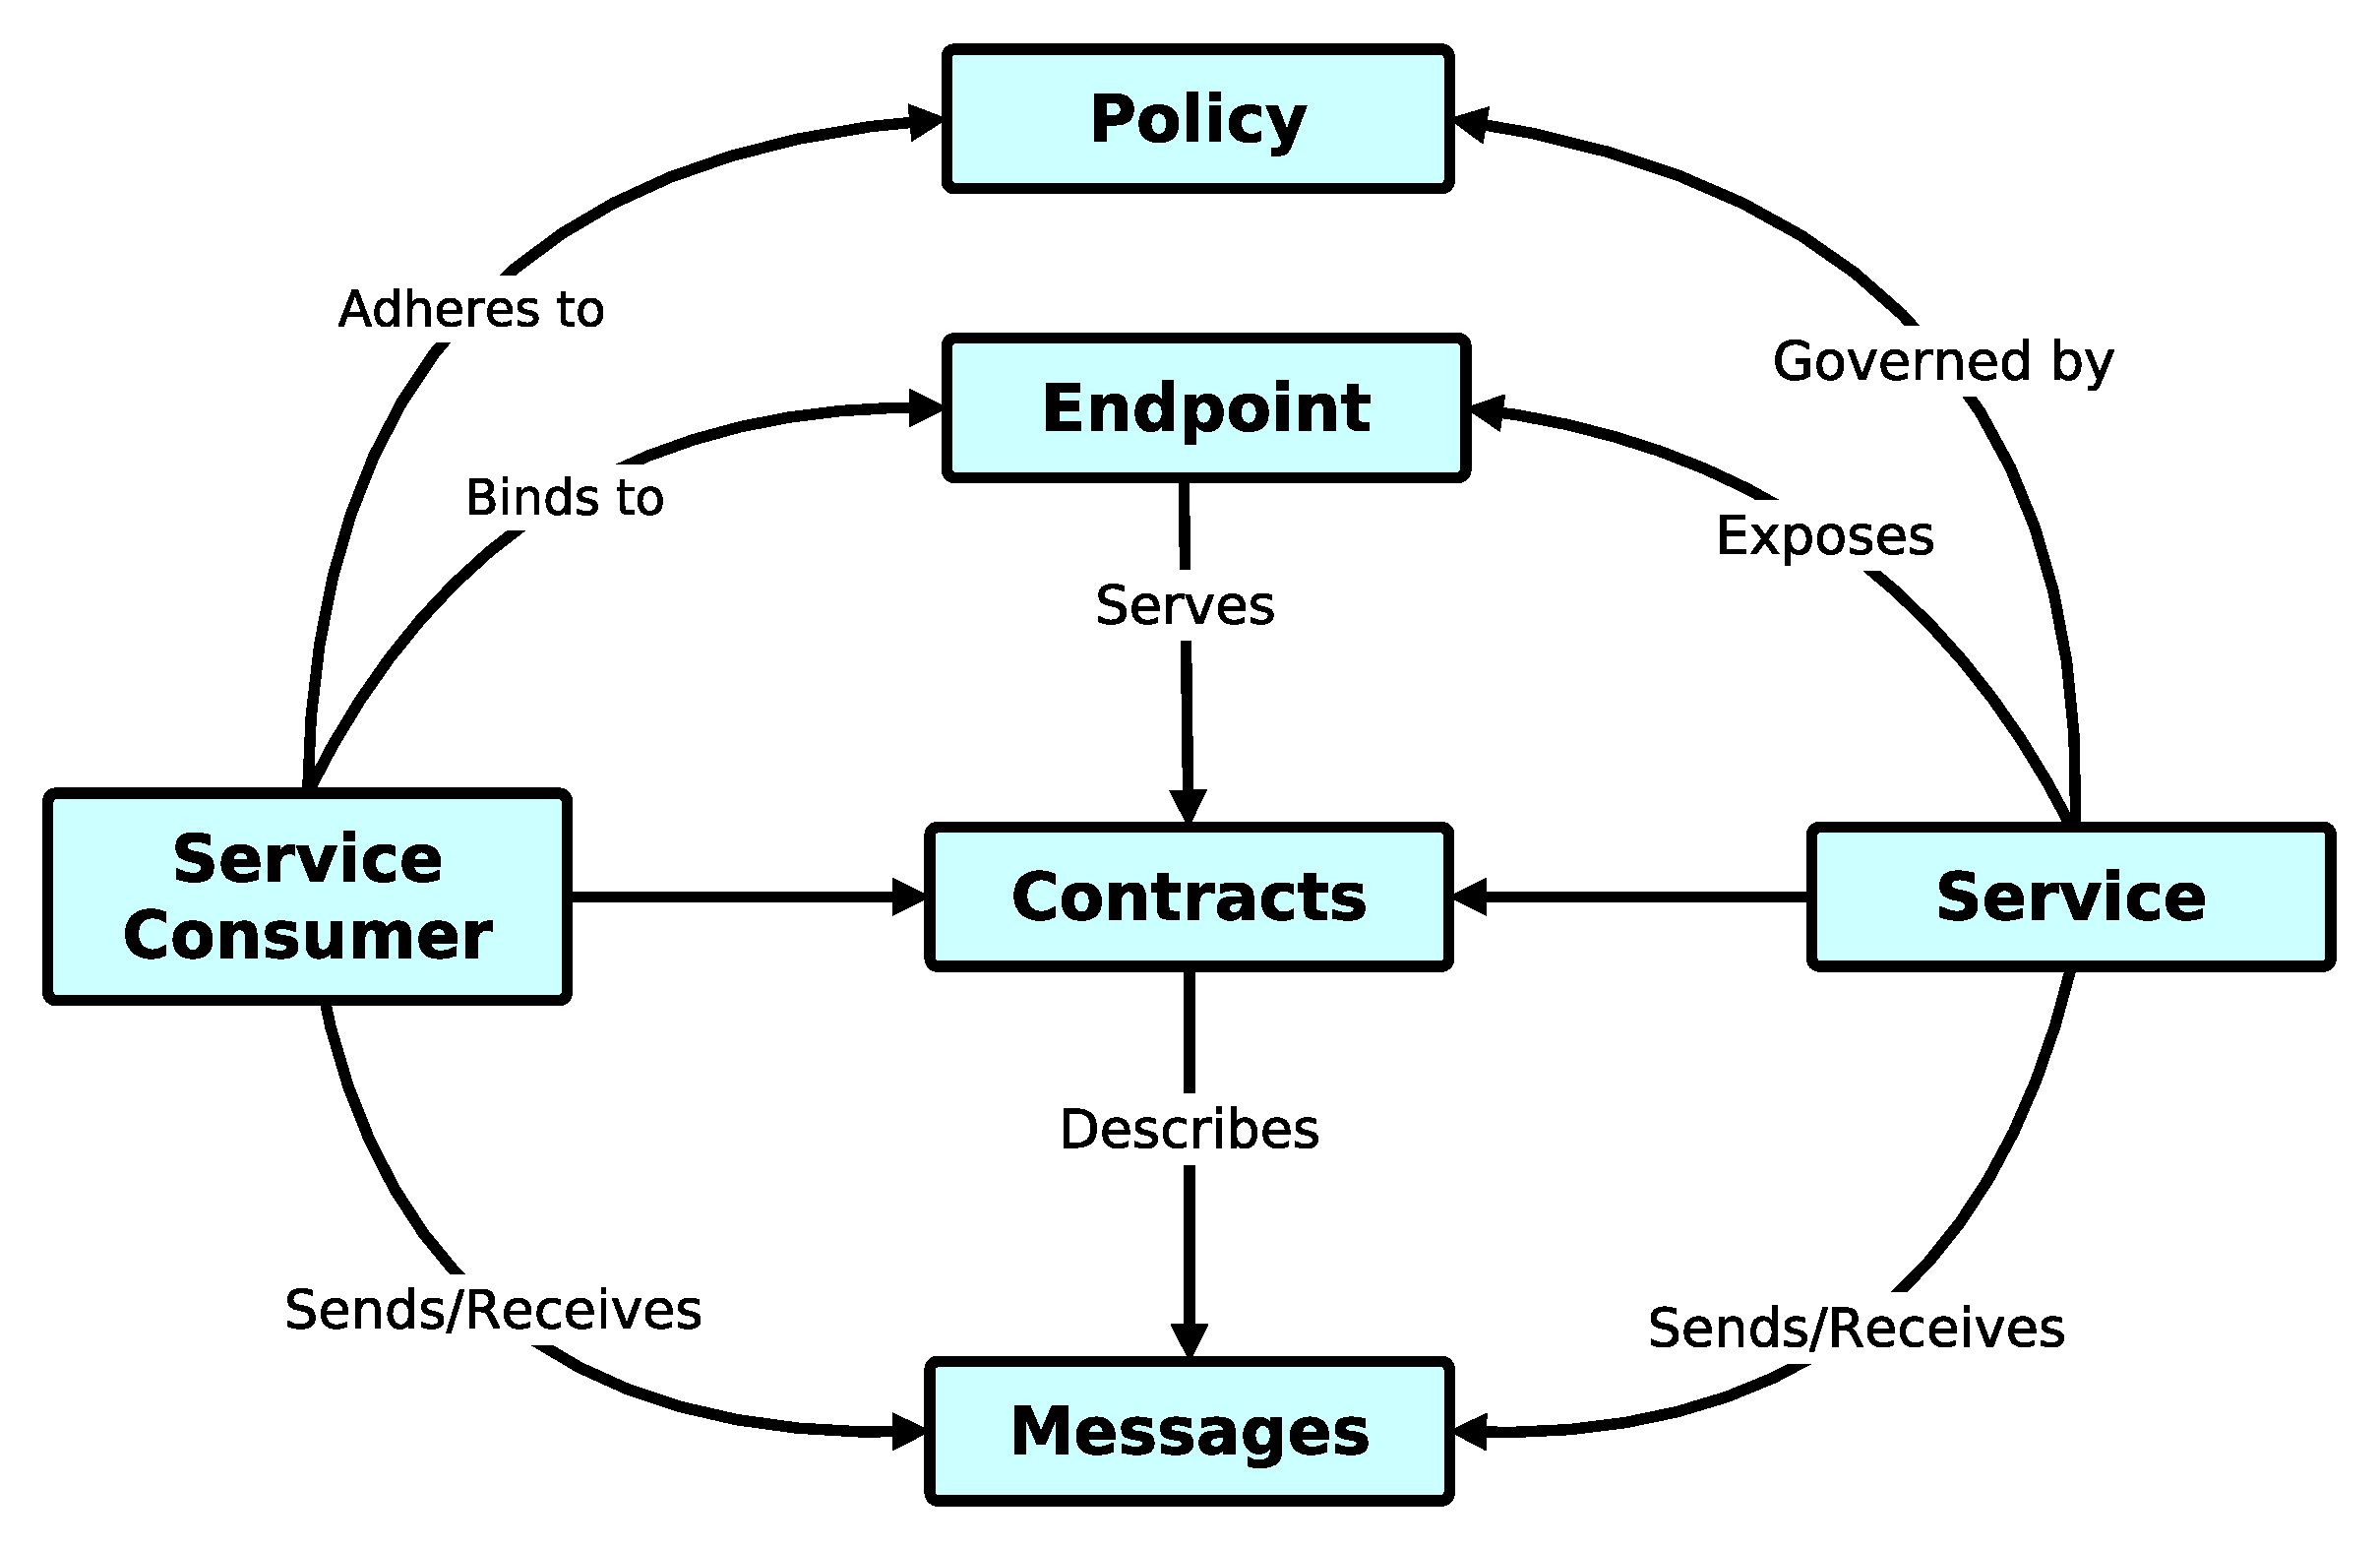
\includegraphics[scale=.2]{img/soa_relation.eps}
\caption{SOA service to consumer}
\label{fig:cm}
\end{figure}




\begin{figure}[!h]
\centering
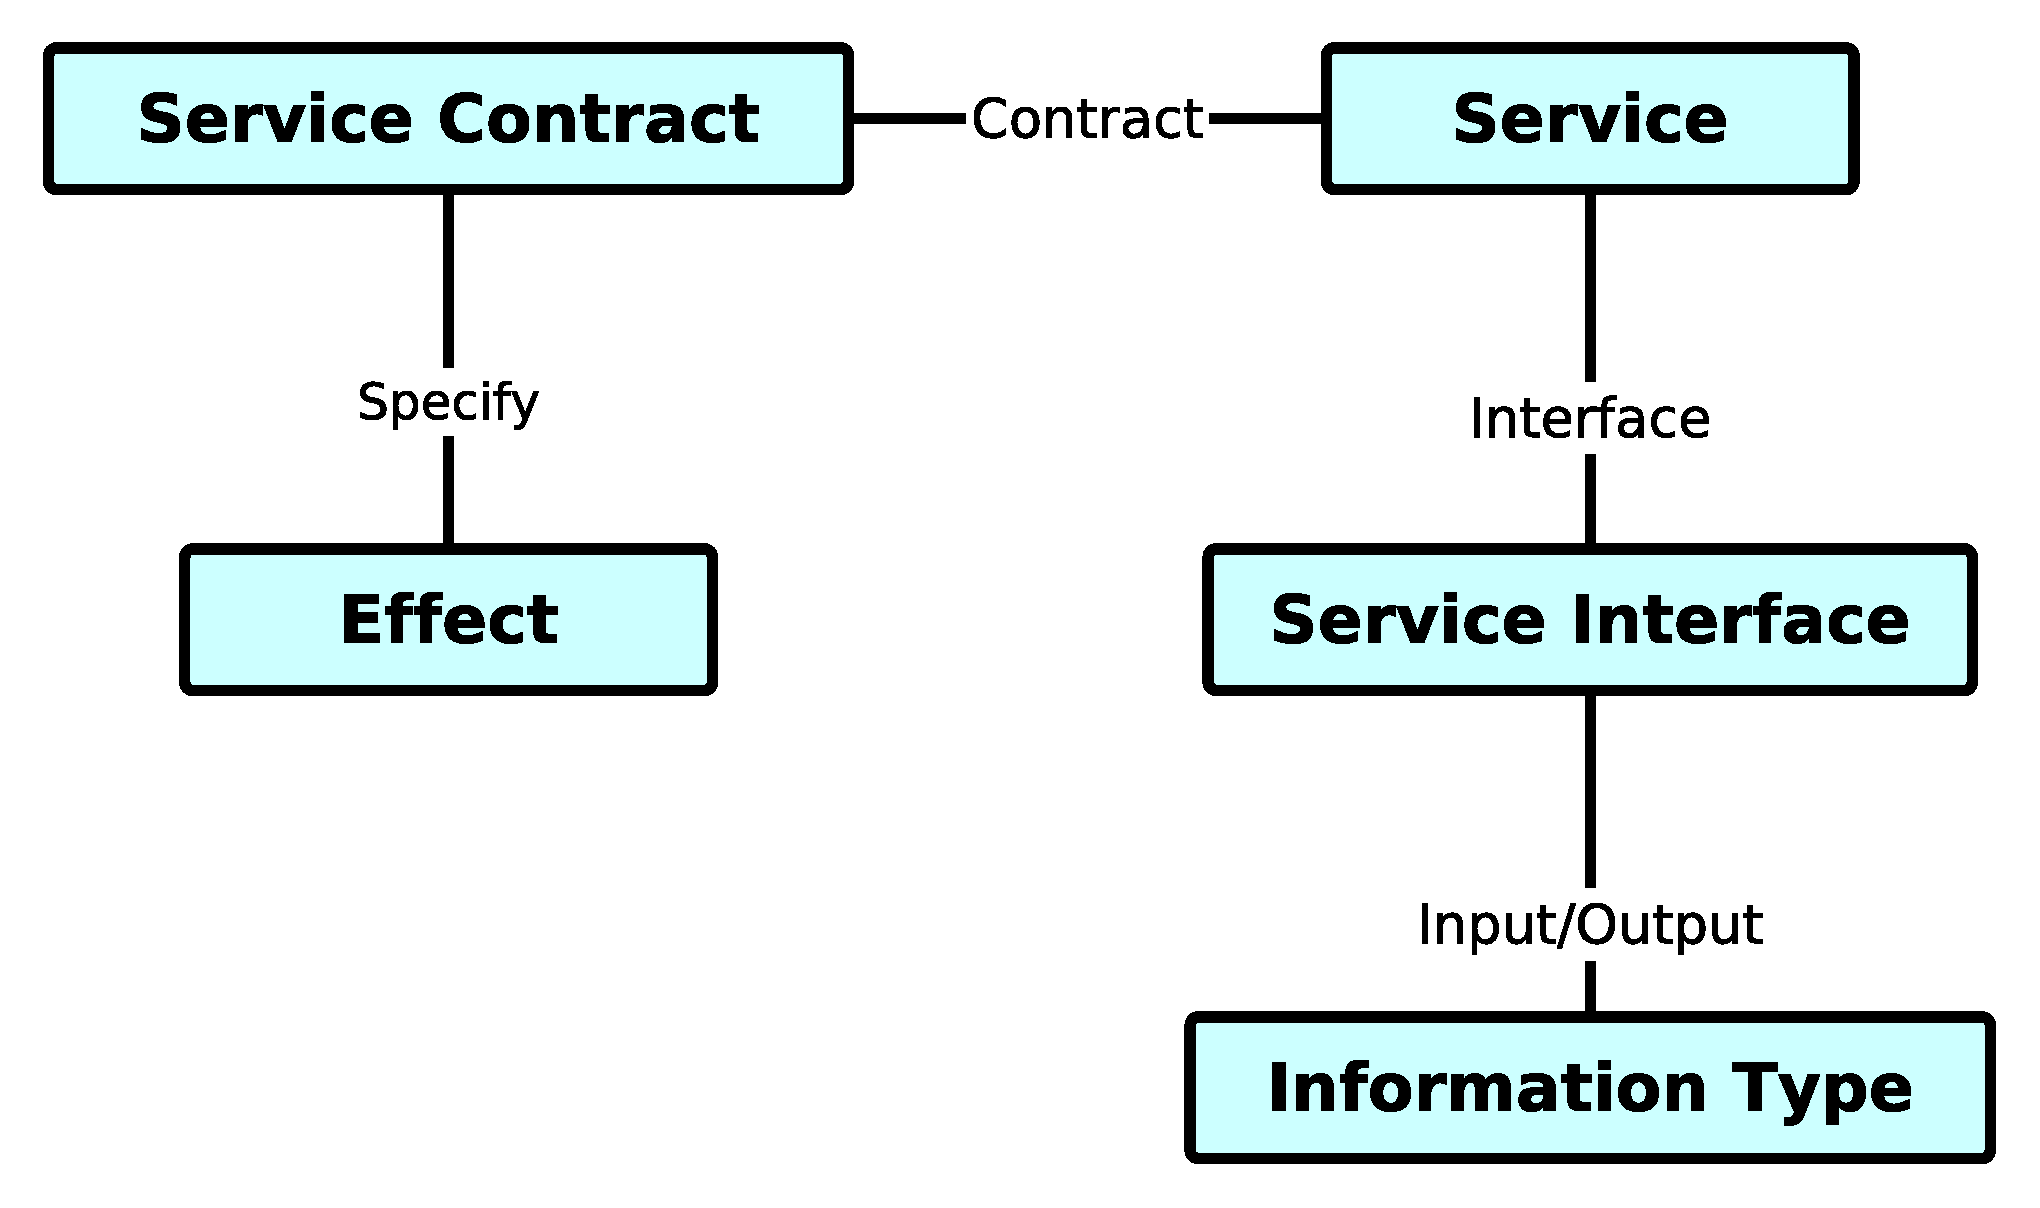
\includegraphics[scale=.2]{img/soa_property.eps}
\caption{SOA service properties}
\label{fig:cm}
\end{figure}

\subsection{Reasoning}

Deployment bez implementačních chyb.

\subsubsection{Model Integrity Validation}

Validace celého řešení vůči high level modelu.

\subsection{External Node Classification}

Mapování vybraného formátu na OpenStack

(HA architektura SDN controller)

\begin{figure}[!h]
\centering
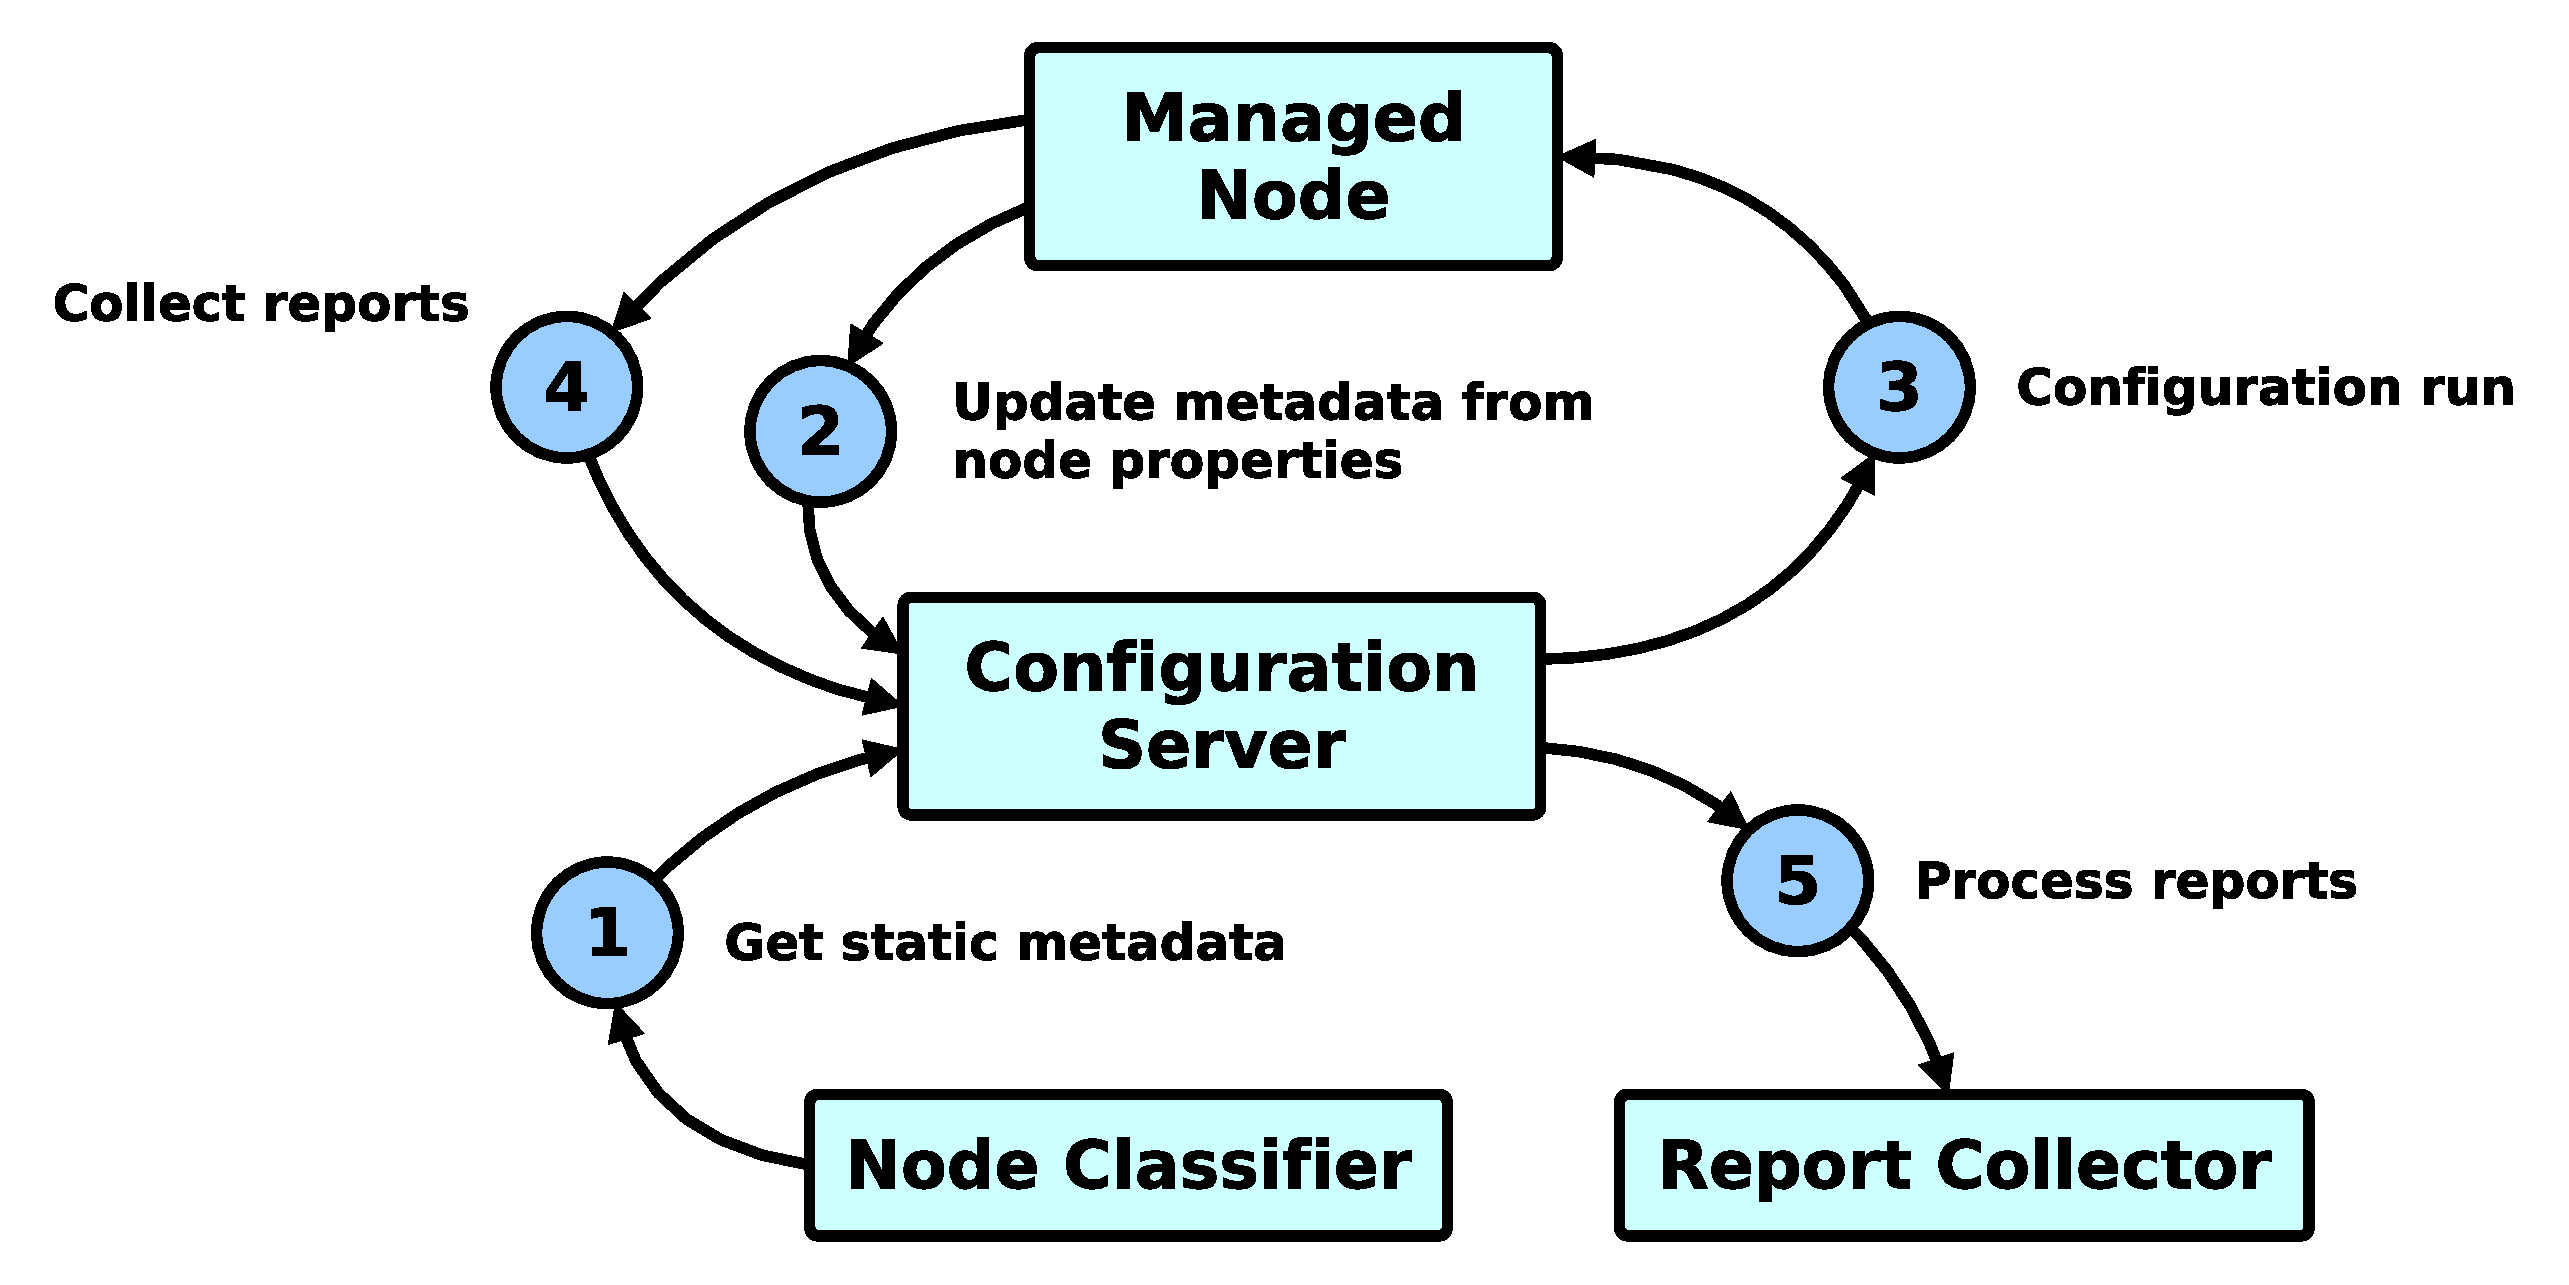
\includegraphics[scale=.15]{img/cm_cycle.eps}
\caption{Configuration Management deployment cycle}
\label{fig:cm}
\end{figure}

\subsubsection{Puppet ENC}

\subsubsection{SaltStack ENC}

Reálný přínos celého řešení


\section{Conclusion}

We have managed to do the first steps in formalization of IaaS Architecture high level models. The representation of models, the ontologies, can be used to create and validate meta-data for individual OpenStack cloud installations. The ontology provides schema for the meta-data for each installation so the overall service integrity is ensured.

We created a python-based web service django-enc that use data from the ontology to generate the suitable meta-data for configuration management tools. The service provide simple interface for manipulating the ontology as well as interfaces for ontology editors. The ontology defines the basic services of OpenStack Havana and Icehouse versions. New components and service backends can be easily defined and included.

% Ontologická reprezentace prostředí, která je vhodná pro agentové prostředí, aby bylo možné provádět autonomní rozhodnutí. 

%\subsection{Future work}

We plan to expand  ontology from virtual and physical servers to network and storage resources by better adoption of configuration management tools. Ontology model is suitable for software agent processing and their rational decisions. It is possible to define agents that will maintain the state of services according to the high-level model. The more parts of the process are modelled and their deployment automated the more manageable the whole system becomes.

\subsubsection*{Acknowledgments.}
 
The paper is supported by the project of specific science Smart networking \& cloud computing solutions (FIM, UHK, SPEV 2015).



\section*{Acknowledgment}

This paper is published thanks to the financial support of the European Operational Programme Education for Competitiveness project INDOP CZ.1.07/2.3.00/45.0014 and UHK specific research project no. 2101.


\begin{thebibliography}{1}


% http://ryandlane.com/blog/2014/08/04/moving-away-from-puppet-saltstack-or-ansible/

% http://ryandlane.com/blog/2014/08/26/saltstack-masterless-bootstrapping/

\bibitem{NIST}
\newblock {\em  NIST. The NIST Definition of Cloud Computing}
\newblock http://csrc.nist.gov/publications/nistpubs/800-145/SP800-145.pdf

\bibitem{CloudServices}
Ivan Ivanov, Marten van Sinderen and Boris Shishkov, editors.
\newblock {\em Cloud Computing and Services Science }
\newblock Springer Science, 978-1461423256, New York, USA, 2012

\bibitem{OpenStackFuel}
\newblock {\em OpenStack. Fuel Wiki }
\newblock https://wiki.openstack.org/wiki/Fuel

\bibitem{CloudStack}
\newblock {\em CloudStack. Open Source Cloud Computing: Apache CloudStack}
\newblock http://cloudstack.apache.org/about.html

\bibitem{DevStack}
\newblock {\em Fedora Project. OpenStack devstack}
\newblock http://fedoraproject.org/wiki/OpenStack\_devstack

\bibitem{ReClass}
\newblock {\em reclass. Recursive external node classification }
\newblock http://reclass.pantsfullofunix.net/

\bibitem{Cfengine}
\newblock {\em CFEngine. FCEngine 3.5 Dcoumentation }
\newblock https://cfengine.com/docs/3.5/index.html

\bibitem{PuppetHiera}
\newblock {\em Puppet Labs. Creating Hierarchies }
\newblock http://docs.puppetlabs.com/hiera/1/hierarchy.html

\bibitem{ForemanCompute}
\newblock {\em The Foreman. The Manual: Compute Resources }
\newblock http://theforeman.org/manuals/1.4/index.html\# 5.2ComputeResources

  
\end{thebibliography}

\end{document}
